\documentclass[12pt,a4paper]{article}

\usepackage{fontspec}
\usepackage{polyglossia}
\setmainlanguage{russian}
\setotherlanguage{english}
\setmainfont{PT Serif}
\newfontfamily\cyrillicfont{PT Serif}
\setsansfont{Arial}
\setmonofont{Courier New}
\newfontfamily\cyrillicfonttt{Courier New}

\usepackage{amsmath,amssymb,mathtools}
\usepackage{geometry}
\usepackage{graphicx}
\usepackage{booktabs}
\usepackage{float}
\usepackage{subcaption}
\usepackage{hyperref}
\usepackage{xcolor}
\usepackage{microtype}

\geometry{left=24mm,right=22mm,top=22mm,bottom=24mm}
\graphicspath{{figures/}{../figures/}}
\captionsetup{font=small,labelfont=bf}
\hypersetup{
    colorlinks=true,
    linkcolor=blue!50!black,
    urlcolor=blue!50!black,
    citecolor=blue!50!black
}
\setlength{\parindent}{1.25cm}
\setlength{\parskip}{0.18em}
\linespread{1.06}
\emergencystretch=2em
\sloppy

\newcommand{\dd}{\,\mathrm{d}}
\newcommand{\ii}{\mathrm{i}}
\newcommand{\e}{\mathrm{e}}
\newcommand{\FT}{\mathcal{F}}
\newcommand{\IFT}{\mathcal{F}^{-1}}

\begin{document}

\begin{titlepage}
\centering
\vspace*{12mm}
\rule{\textwidth}{0.7pt}\par
\vspace{8mm}
{\Large Учебно-исследовательский отчет на вопрос по выбору\par}
\vspace{24mm}
{\huge\bfseries Саморепродукция периодических структур\par}
\vspace{3mm}
{\huge\bfseries в ближнем поле\par}
\vspace{8mm}
{\Large Эффект Талбота для амплитудной и фазовой решетки\par}
\vspace{10mm}
\rule{0.66\textwidth}{0.45pt}\par
\vspace{15mm}
\begin{flushright}
{\large Выполнила:\par}
{\Large Щербухина Анастасия Викторовна\par}
{\large 2 курс ФПМИ\par}
\end{flushright}
\vfill
{\large МФТИ, 2026\par}
\vspace{6mm}
\rule{\textwidth}{0.7pt}\par
\end{titlepage}

\tableofcontents
\newpage

\begin{abstract}
В работе изучается эффект Талбота: самовоспроизведение периодических структур при дифракции Френеля. Рассмотрены амплитудные, фазовые и смешанные решетки. Получены основные теоретические формулы, включая параксиальное волновое уравнение, спектральный пропагатор, длину Талбота $z_T=2d^2/\lambda$, сдвиг изображения при $z_T/2$, дробные изображения и точную модель углового спектра. Реализована численная модель на основе дискретного преобразования Фурье, построены ковры Талбота для разных типов решеток, проведены проверки корректности и сравнение параксиальной и точной моделей.
\end{abstract}

\section{Постановка задачи и мотивация}

Пусть на тонкую периодическую структуру с периодом $d$ нормально падает плоская волна одной длины волны $\lambda$. Экспериментально оказывается, что в ближнем поле за решеткой на специальных расстояниях возникают изображения, повторяющие исходную периодическую структуру. Это явление называется эффектом Талбота.

Цель работы состоит в том, чтобы связать физический механизм эффекта Талбота с его численным моделированием. Для этого в отчете выводится параксиальная модель, строится спектральный алгоритм распространения, сравниваются амплитудные и фазовые решетки, а также проверяется, где параксиальное приближение начинает отличаться от точной угловой модели. Отдельное внимание уделено самим картинам интенсивности: по ним видно восстановление структуры, сдвиг на половине длины Талбота и появление дробных изображений.

Работа связана с темами курса оптики: дифракция на тонком экране, дифракция Френеля, дифракция Фраунгофера, фурье-оптика, периодические структуры, амплитудные и фазовые решетки.

\section{Теоретическая модель}

\subsection{Тонкая периодическая решетка}

Рассмотрим комплексную амплитуду монохроматического поля $U(x,z)$. Физическое поле можно записать как
\begin{equation}
    E(x,z,t)=\operatorname{Re}\{U(x,z)\e^{-\ii\omega t}\}.
\end{equation}

Тонкая решетка, расположенная в плоскости $z=0$, задается комплексной функцией пропускания $t(x)$:
\begin{equation}
    U(x,0)=t(x)U_{\mathrm{in}}.
\end{equation}
Для нормированной падающей плоской волны положим $U_{\mathrm{in}}=1$, тогда
\begin{equation}
    U(x,0)=t(x).
\end{equation}

Периодичность означает
\begin{equation}
    t(x+d)=t(x).
\end{equation}
Поэтому $t(x)$ раскладывается в ряд Фурье:
\begin{equation}
    t(x)=\sum_{m=-\infty}^{\infty} c_m
    \e^{\ii(2\pi m/d)x},
    \label{eq:fourier_series}
\end{equation}
где коэффициенты
\begin{equation}
    c_m=\frac{1}{d}\int_0^d t(x)
    \e^{-\ii(2\pi m/d)x}\dd x.
\end{equation}
Каждый член ряда соответствует дифракционному порядку с поперечным волновым числом
\begin{equation}
    k_{x,m}=\frac{2\pi m}{d}.
\end{equation}

\subsection{Амплитудная и фазовая решетки}

Амплитудная решетка изменяет модуль поля:
\begin{equation}
    t_A(x)=a(x), \qquad 0\le a(x)\le 1.
\end{equation}
Например, бинарная амплитудная решетка с коэффициентом заполнения $\alpha$:
\begin{equation}
    \xi=x-d\left\lfloor\frac{x}{d}\right\rfloor,\qquad 0\le \xi<d,
\end{equation}
\begin{equation}
    t_A(x)=
    \begin{cases}
        1, & 0 < \xi < \alpha d,\\
        0, & \alpha d < \xi < d.
    \end{cases}
\end{equation}
Она сразу создает контраст интенсивности:
\begin{equation}
    I(x,0)=|t_A(x)|^2.
\end{equation}

Фазовая решетка меняет фазу, но в идеале не меняет модуль:
\begin{equation}
    t_\phi(x)=\exp(\ii\phi(x)).
\end{equation}
Для такой решетки
\begin{equation}
    |t_\phi(x)|^2=1,
\end{equation}
поэтому сразу после решетки интенсивность может быть почти постоянной. Тем не менее фаза периодична, а при распространении фазовая модуляция превращается в модуляцию интенсивности вследствие интерференции дифракционных порядков.

\subsection{Параксиальное приближение для медленно меняющейся огибающей}

Скалярная комплексная амплитуда в однородной среде удовлетворяет уравнению Гельмгольца:
\begin{equation}
    \nabla^2 U+k^2U=0,
    \qquad
    k=\frac{2\pi}{\lambda}.
    \label{eq:helmholtz}
\end{equation}
В двумерном случае $(x,z)$:
\begin{equation}
    \frac{\partial^2 U}{\partial x^2}
    +\frac{\partial^2 U}{\partial z^2}
    +k^2U=0.
\end{equation}

Если поле распространяется преимущественно вдоль $z$, удобно выделить быстро осциллирующий множитель:
\begin{equation}
    U(x,z)=\psi(x,z)\e^{\ii kz},
\end{equation}
Здесь медленно меняющаяся комплексная огибающая обозначена как $\psi(x,z)$; она содержит поперечную структуру пучка и ее медленную эволюцию вдоль $z$, а быстрые колебания плоской несущей волны вынесены в множитель $\e^{\ii kz}$. Производные по $z$:
\begin{align}
    \frac{\partial U}{\partial z}
    &=\e^{\ii kz}\left(\frac{\partial\psi}{\partial z}+\ii k\psi\right),\\
    \frac{\partial^2 U}{\partial z^2}
    &=\e^{\ii kz}\left(
    \frac{\partial^2\psi}{\partial z^2}
    +2\ii k\frac{\partial\psi}{\partial z}
    -k^2\psi
    \right).
\end{align}
Подстановка в \eqref{eq:helmholtz} дает
\begin{equation}
    \frac{\partial^2\psi}{\partial x^2}
    +\frac{\partial^2\psi}{\partial z^2}
    +2\ii k\frac{\partial\psi}{\partial z}=0.
\end{equation}

Параксиальное приближение состоит в условии медленного изменения огибающей вдоль $z$:
\begin{equation}
    \left|\frac{\partial^2\psi}{\partial z^2}\right|
    \ll
    \left|2k\frac{\partial\psi}{\partial z}\right|.
\end{equation}
Тогда получаем параксиальное волновое уравнение
\begin{equation}
    2\ii k\frac{\partial\psi}{\partial z}
    +\frac{\partial^2\psi}{\partial x^2}=0,
\end{equation}
или
\begin{equation}
    \ii\frac{\partial\psi}{\partial z}
    =
    -\frac{1}{2k}\frac{\partial^2\psi}{\partial x^2}.
    \label{eq:paraxial}
\end{equation}
Это уравнение математически аналогично уравнению Шредингера для свободной частицы: роль времени играет координата $z$.

\subsection{Спектральное решение и связь с дифракцией Френеля}

Разложим огибающую в интеграл Фурье:
\begin{equation}
    \psi(x,0)=\frac{1}{2\pi}\int_{-\infty}^{\infty}
    \widehat{\psi}(k_x,0)\e^{\ii k_xx}\dd k_x.
\end{equation}
Для одной гармоники $\psi=A(z)\e^{\ii k_xx}$ подстановка в \eqref{eq:paraxial} дает
\begin{equation}
    \ii\frac{\dd A}{\dd z}=\frac{k_x^2}{2k}A.
\end{equation}
Отсюда
\begin{equation}
    A(z)=A(0)\e^{-\ii(k_x^2/2k)z}.
\end{equation}
Следовательно,
\begin{equation}
    \widehat{\psi}(k_x,z)=
    \widehat{\psi}(k_x,0)
    \e^{-\ii(k_x^2/2k)z}.
    \label{eq:paraxial_propagator}
\end{equation}

В координатном пространстве это эквивалентно интегралу Френеля:
\begin{equation}
    \psi(x,z)=
    \sqrt{\frac{k}{2\pi \ii z}}
    \int_{-\infty}^{\infty}
    \psi(x',0)
    \e^{\ii k(x-x')^2/(2z)}\dd x'.
    \label{eq:fresnel_integral}
\end{equation}
Таким образом, эффект Талбота является ближнепольным эффектом дифракции Френеля.

\subsection{Вывод длины Талбота}

Пусть поле сразу после решетки задано рядом \eqref{eq:fourier_series}:
\begin{equation}
    \psi(x,0)=
    \sum_{m=-\infty}^{\infty} c_m
    \e^{\ii(2\pi m/d)x}.
\end{equation}
Для $m$-го порядка
\begin{equation}
    k_{x,m}=\frac{2\pi m}{d}.
\end{equation}
Используя \eqref{eq:paraxial_propagator}, получаем
\begin{align}
    \psi(x,z)
    &=
    \sum_m c_m
    \e^{\ii(2\pi m/d)x}
    \e^{-\ii(1/2k)(2\pi m/d)^2z}.
\end{align}
Так как $k=2\pi/\lambda$, фазовый множитель равен
\begin{equation}
    \e^{-\ii\pi m^2\lambda z/d^2}.
    \label{eq:talbot_phase}
\end{equation}

Полное самовоспроизведение требует, чтобы для всех целых $m$
\begin{equation}
    \e^{-\ii\pi m^2\lambda z/d^2}=1.
\end{equation}
Минимальное положительное расстояние, на котором это выполняется:
\begin{equation}
    z_T=\frac{2d^2}{\lambda}.
    \label{eq:talbot_length}
\end{equation}
Действительно,
\begin{equation}
    \e^{-\ii\pi m^2\lambda z_T/d^2}
    =
    \e^{-\ii 2\pi m^2}=1.
\end{equation}
Поэтому
\begin{equation}
    \psi(x,z_T)=\psi(x,0)
\end{equation}
с точностью до общего фазового множителя, если работать с полным полем $U$.

\subsection{Половина длины Талбота и сдвиг на половину периода}

При $z=z_T/2=d^2/\lambda$ фазовый множитель \eqref{eq:talbot_phase} становится
\begin{equation}
    \e^{-\ii\pi m^2}.
\end{equation}
Для целого $m$ числа $m$ и $m^2$ имеют одинаковую четность, поэтому
\begin{equation}
    \e^{-\ii\pi m^2}=\e^{-\ii\pi m}=(-1)^m.
\end{equation}
Но
\begin{equation}
    (-1)^m=\e^{-\ii(2\pi m/d)(d/2)}.
\end{equation}
Тогда
\begin{align}
    \psi(x,z_T/2)
    &=
    \sum_m c_m
    \e^{\ii(2\pi m/d)x}
    \e^{-\ii\pi m}\\
    &=
    \sum_m c_m
    \e^{\ii(2\pi m/d)(x-d/2)}\\
    &=\psi(x-d/2,0).
\end{align}
Итак, на половине длины Талбота изображение восстанавливается со сдвигом на $d/2$:
\begin{equation}
    I(x,z_T/2)=I(x-d/2,0).
\end{equation}

\subsection{Дробные изображения}

На рациональных долях длины Талбота
\begin{equation}
    z=\frac{p}{q}z_T,\qquad (p,q)=1,
\end{equation}
фазовый множитель имеет вид
\begin{equation}
    \e^{-\ii 2\pi(p/q)m^2}.
\end{equation}
Он периодичен по номеру порядка $m$ с некоторым периодом $Q$, равным $q$ или $2q$ в зависимости от четности. Поэтому поле можно представить как конечную сумму сдвинутых копий исходного поля:
\begin{equation}
    \psi\left(x,\frac{p}{q}z_T\right)
    =
    \sum_{r=0}^{Q-1} a_r
    \psi\left(x-\frac{rd}{Q},0\right),
\end{equation}
где коэффициенты $a_r$ выражаются через гауссовы суммы:
\begin{equation}
    a_r=
    \frac{1}{Q}
    \sum_{m=0}^{Q-1}
    \e^{-\ii 2\pi(p/q)m^2}
    \e^{\ii 2\pi mr/Q}.
\end{equation}
На картинах интенсивности это проявляется как дробные изображения и более мелкая периодическая структура внутри исходного периода.

\subsection{Точная модель углового спектра}

Параксиальная теория использует приближение малых углов. Более точная скалярная модель раскладывает поле в плоские волны:
\begin{equation}
    U(x,0)=\frac{1}{2\pi}\int
    \widehat U(k_x,0)\e^{\ii k_xx}\dd k_x.
\end{equation}
Для каждой компоненты
\begin{equation}
    k_z=\sqrt{k^2-k_x^2}.
\end{equation}
Точное распространение:
\begin{equation}
    \widehat U(k_x,z)=
    \widehat U(k_x,0)
    \e^{\ii z\sqrt{k^2-k_x^2}}.
    \label{eq:exact_propagator}
\end{equation}

Связь с параксиальным приближением получается из разложения:
\begin{equation}
    \sqrt{k^2-k_x^2}
    =
    k\sqrt{1-\frac{k_x^2}{k^2}}
    \approx
    k-\frac{k_x^2}{2k},
    \qquad |k_x|\ll k.
\end{equation}
Тогда
\begin{equation}
    \e^{\ii z\sqrt{k^2-k_x^2}}
    \approx
    \e^{\ii kz}
    \e^{-\ii(k_x^2/2k)z}.
\end{equation}
После выделения несущего множителя $\e^{\ii kz}$ получается параксиальный пропагатор \eqref{eq:paraxial_propagator}.

Если $|k_x|>k$, то
\begin{equation}
    k_z=\ii\sqrt{k_x^2-k^2},
\end{equation}
и множитель распространения содержит экспоненциальное затухание:
\begin{equation}
    \e^{\ii k_zz}=
    \e^{-z\sqrt{k_x^2-k^2}}.
\end{equation}
Такие компоненты называются эванесцентными. Они важны для очень мелких деталей, но быстро исчезают при распространении.

\subsection{Ограничения параксиального приближения}

Для $m$-го дифракционного порядка
\begin{equation}
    \sin\theta_m=\frac{k_{x,m}}{k}=\frac{m\lambda}{d}.
\end{equation}
Параксиальное приближение требует
\begin{equation}
    \left|\frac{m\lambda}{d}\right|\ll 1
\end{equation}
для всех существенных порядков. Если $d$ сравнимо с $\lambda$, высокие порядки идут под большими углами или становятся эванесцентными; тогда точная модель \eqref{eq:exact_propagator} необходима.

\section{Численная реализация и состав проекта}

В работе построена воспроизводимая численная модель эффекта Талбота на Python. Основные компоненты:
\begin{itemize}
    \item модуль решеток: бинарные амплитудные, синусоидальные фазовые, синусоидальные амплитудные, бинарные фазовые, пилообразные фазовые, треугольные амплитудные, многощелевые и смешанные амплитудно-фазовые решетки;
    \item модуль распространения: параксиальный угловой спектр, точный угловой спектр, общий диспетчер моделей;
    \item модуль метрик: корреляция, относительная ошибка $L_2$, полная мощность, корреляция с оптимальным циклическим сдвигом;
    \item скрипт генерации рисунков;
    \item Jupyter-ноутбук для самостоятельного запуска;
    \item автоматические тесты корректности.
\end{itemize}

Все физические величины задаются в СИ. Расчетная сетка по умолчанию:
\begin{table}[H]
\centering
\begin{tabular}{lll}
\toprule
Параметр & Обозначение & Значение\\
\midrule
Длина волны & $\lambda$ & $532\,\text{нм}$\\
Период решетки & $d$ & $40\,\text{мкм}$\\
Длина Талбота & $z_T=2d^2/\lambda$ & $6.02\,\text{мм}$\\
Число периодов & $N_p$ & $64$\\
Число точек по $x$ & $N_x$ & $8192$\\
Число точек по $z$ & $N_z$ & $500$\\
Заполнение амплитудной решетки & $\alpha$ & $0.5$\\
Глубина фазовой решетки & $\phi_0$ & $\pi/2$\\
\bottomrule
\end{tabular}
\caption{Параметры моделирования по умолчанию.}
\end{table}

\subsection{Численный метод}

На равномерной сетке
\begin{equation}
    x_j=\left(j-\frac{N_x}{2}\right)\Delta x
\end{equation}
задается начальное поле $U_j(0)=t(x_j)$. Далее выполняется:
\begin{enumerate}
    \item вычисление спектра $\widehat U(k_x,0)$ через дискретное преобразование Фурье; в программе для скорости используется его быстрый алгоритм;
    \item умножение спектра на параксиальный или точный пропагатор;
    \item обратное дискретное преобразование Фурье;
    \item вычисление интенсивности $I(x,z)=|U(x,z)|^2$.
\end{enumerate}

Параксиальная модель в коде:
\begin{equation}
    H_{\mathrm{par}}(k_x,z)=
    \e^{-\ii(k_x^2/2k)z}.
\end{equation}
Точная модель для огибающей:
\begin{equation}
    H_{\mathrm{exact}}(k_x,z)=
    \e^{\ii z(\sqrt{k^2-k_x^2}-k)}.
\end{equation}
Вычитание $k$ соответствует выделению общей фазы $\e^{\ii kz}$.

\section{Результаты моделирования}

\subsection{Ковры из интерактивного ноутбука}

\begin{figure}[H]
\centering
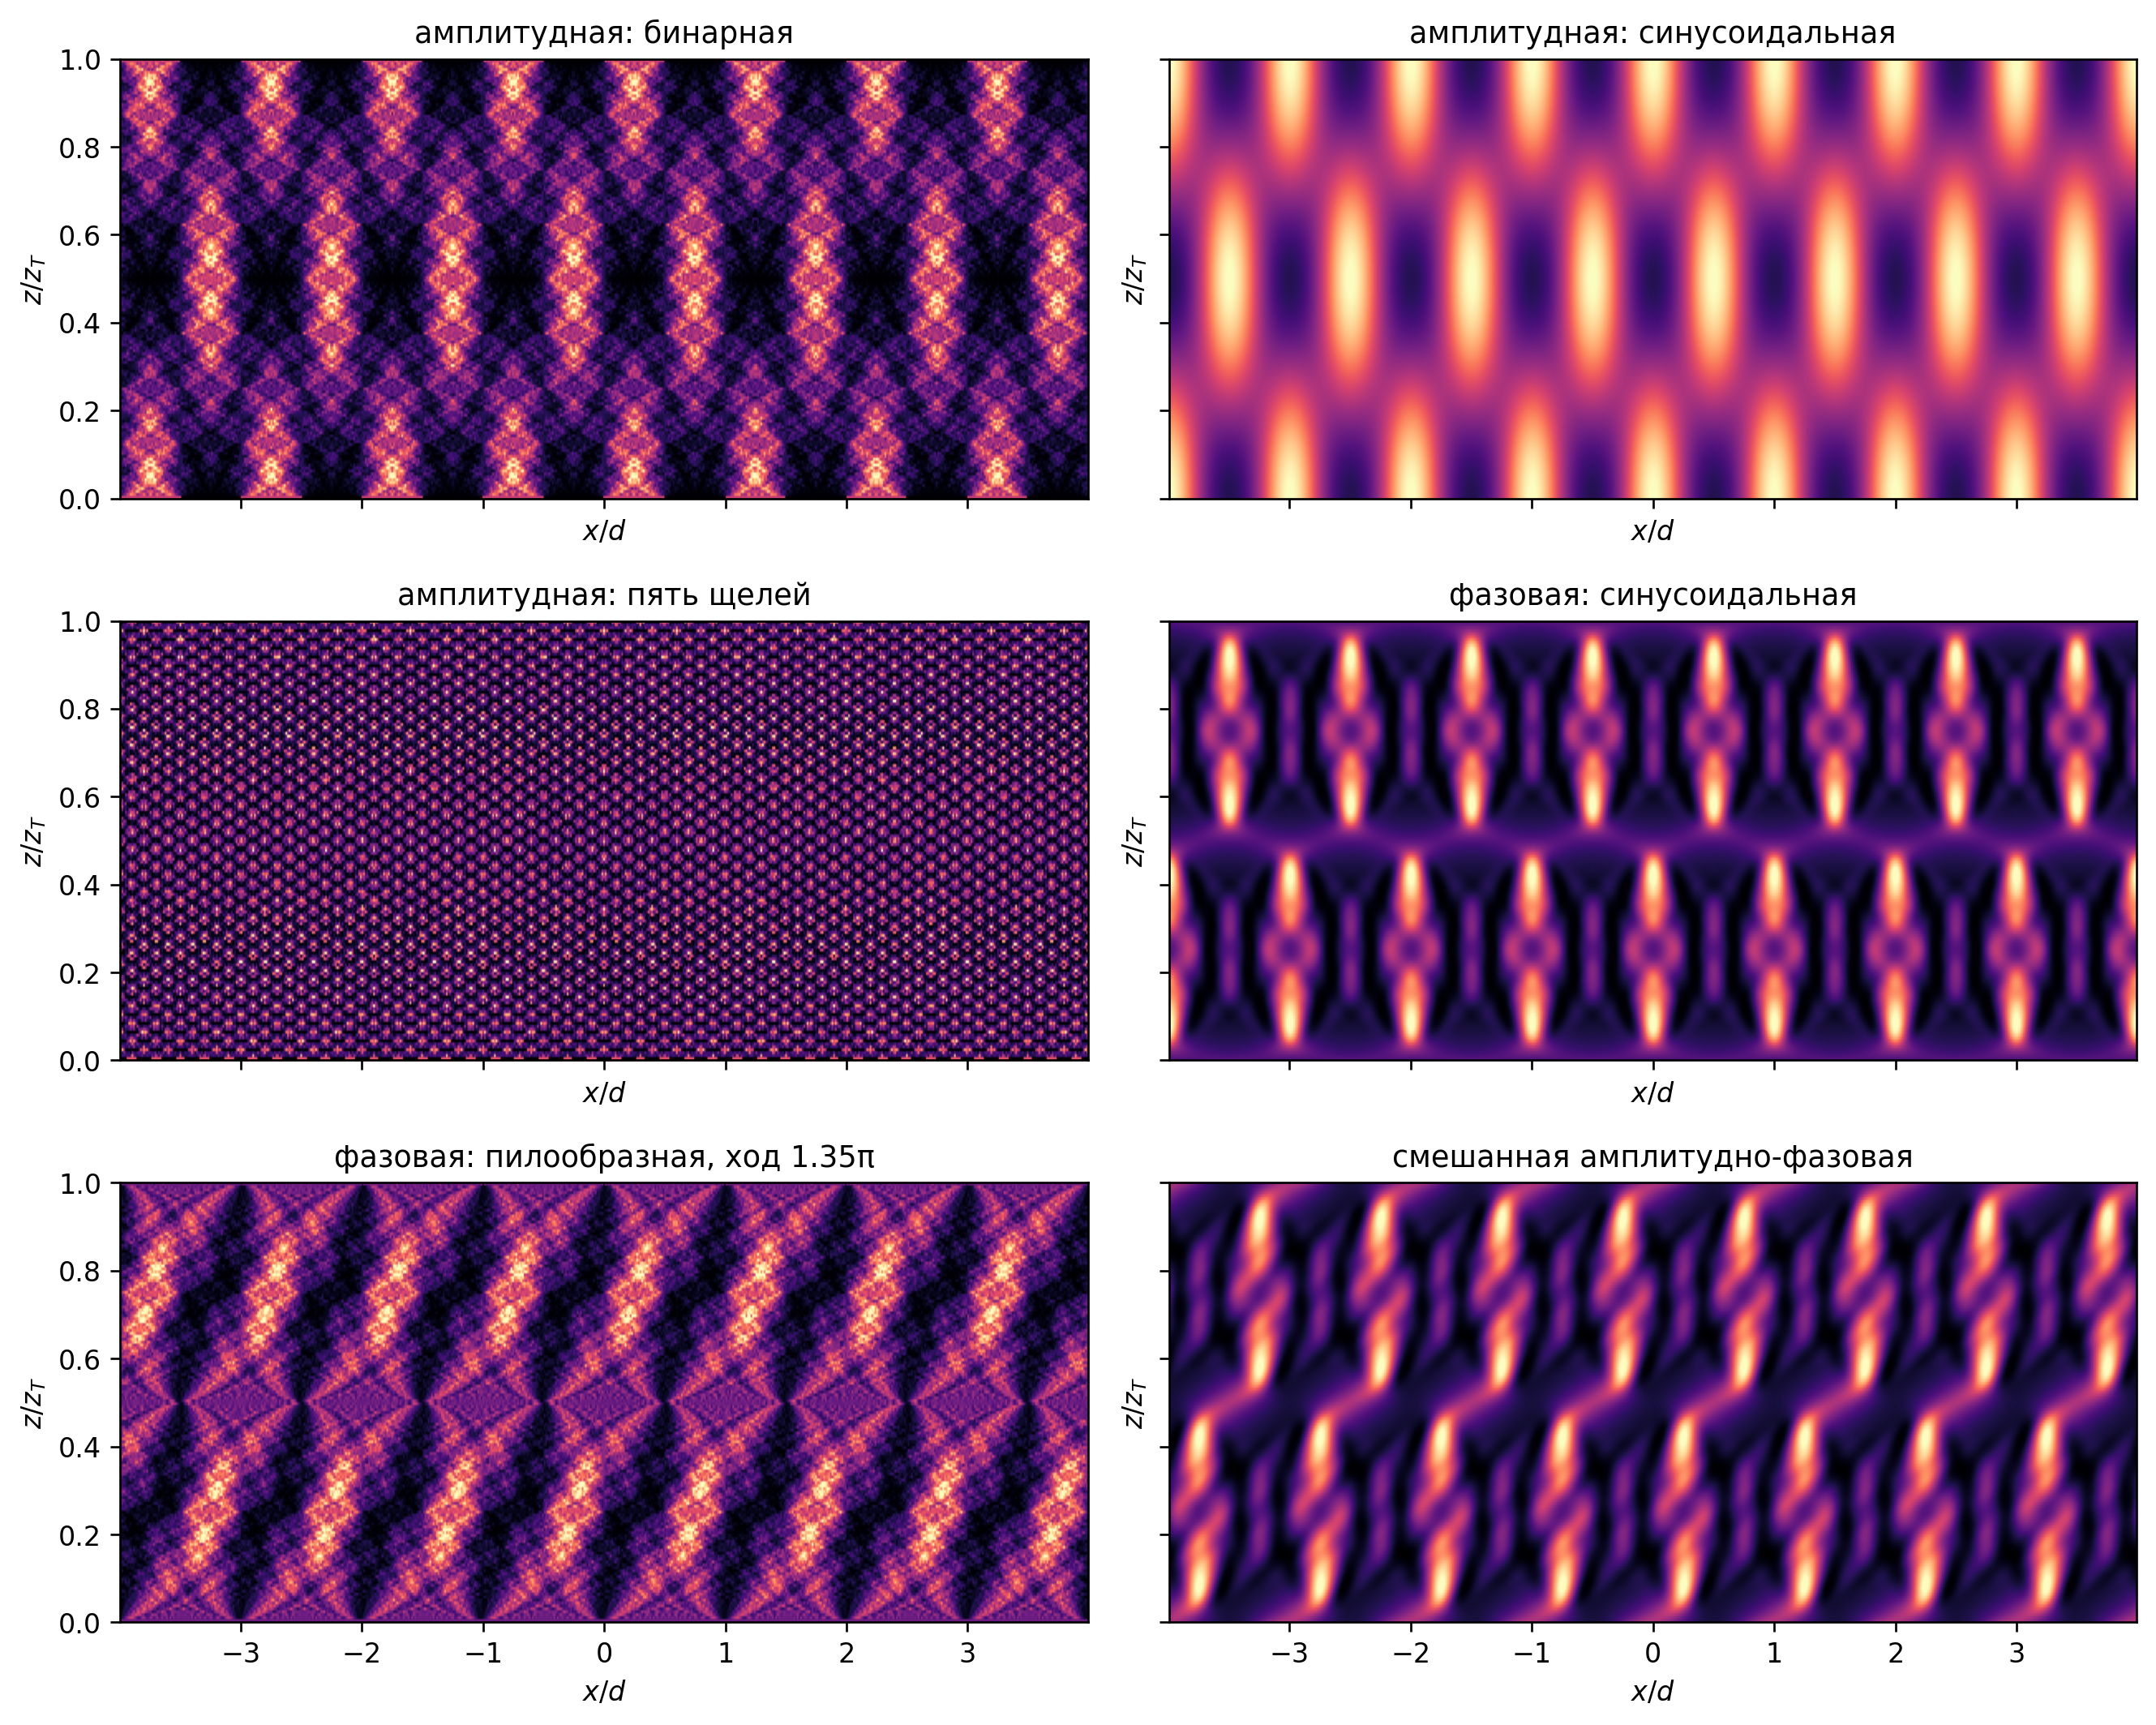
\includegraphics[width=0.98\textwidth]{notebook_shape_gallery.png}
\caption{Галерея ковров Талбота из интерактивного ноутбука. Сравниваются бинарная, синусоидальная и многощелевая амплитудные решетки, синусоидальная и пилообразная фазовые решетки, а также смешанная амплитудно-фазовая структура.}
\end{figure}
\clearpage

\subsection{Многощелевые решетки}

\begin{figure}[H]
\centering
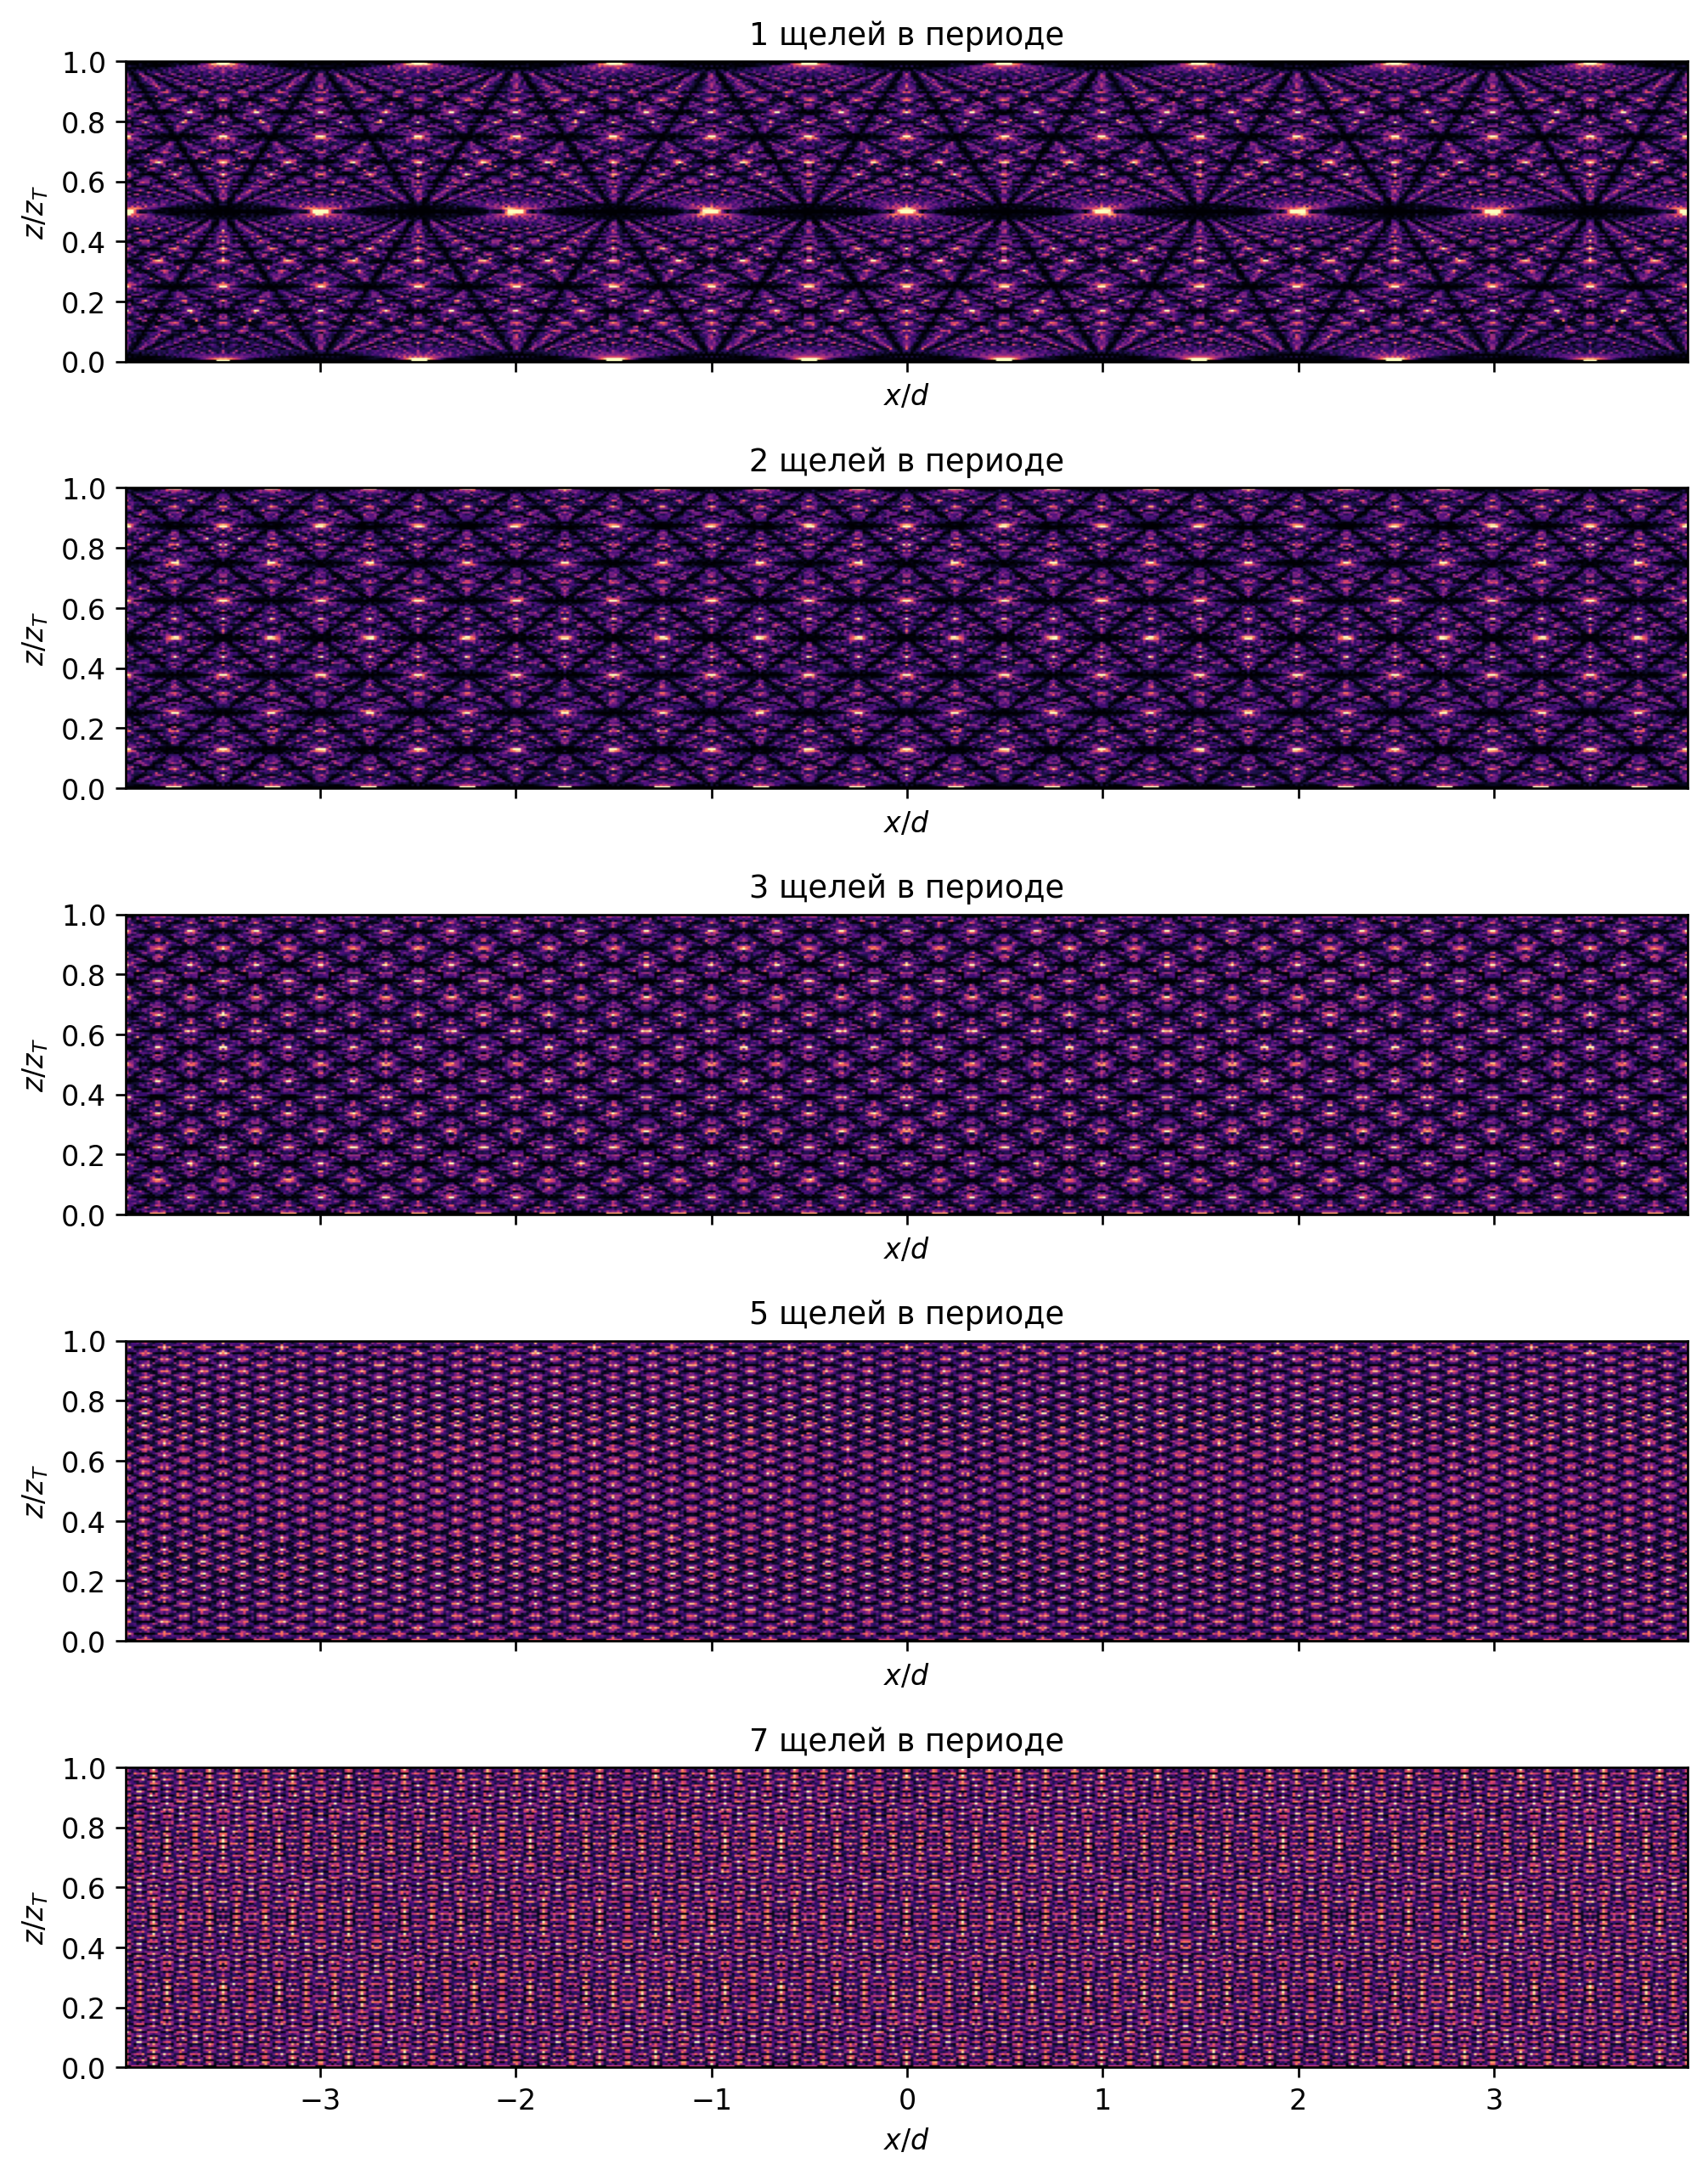
\includegraphics[height=0.84\textheight]{notebook_slit_count_gallery.png}
\caption{Влияние числа щелей внутри одного периода. При увеличении числа отверстий появляется более мелкая внутренняя структура, но масштаб полного самовоспроизведения по-прежнему задается периодом $d$.}
\end{figure}
\clearpage

\subsection{Фазовые решетки}

\begin{figure}[H]
\centering
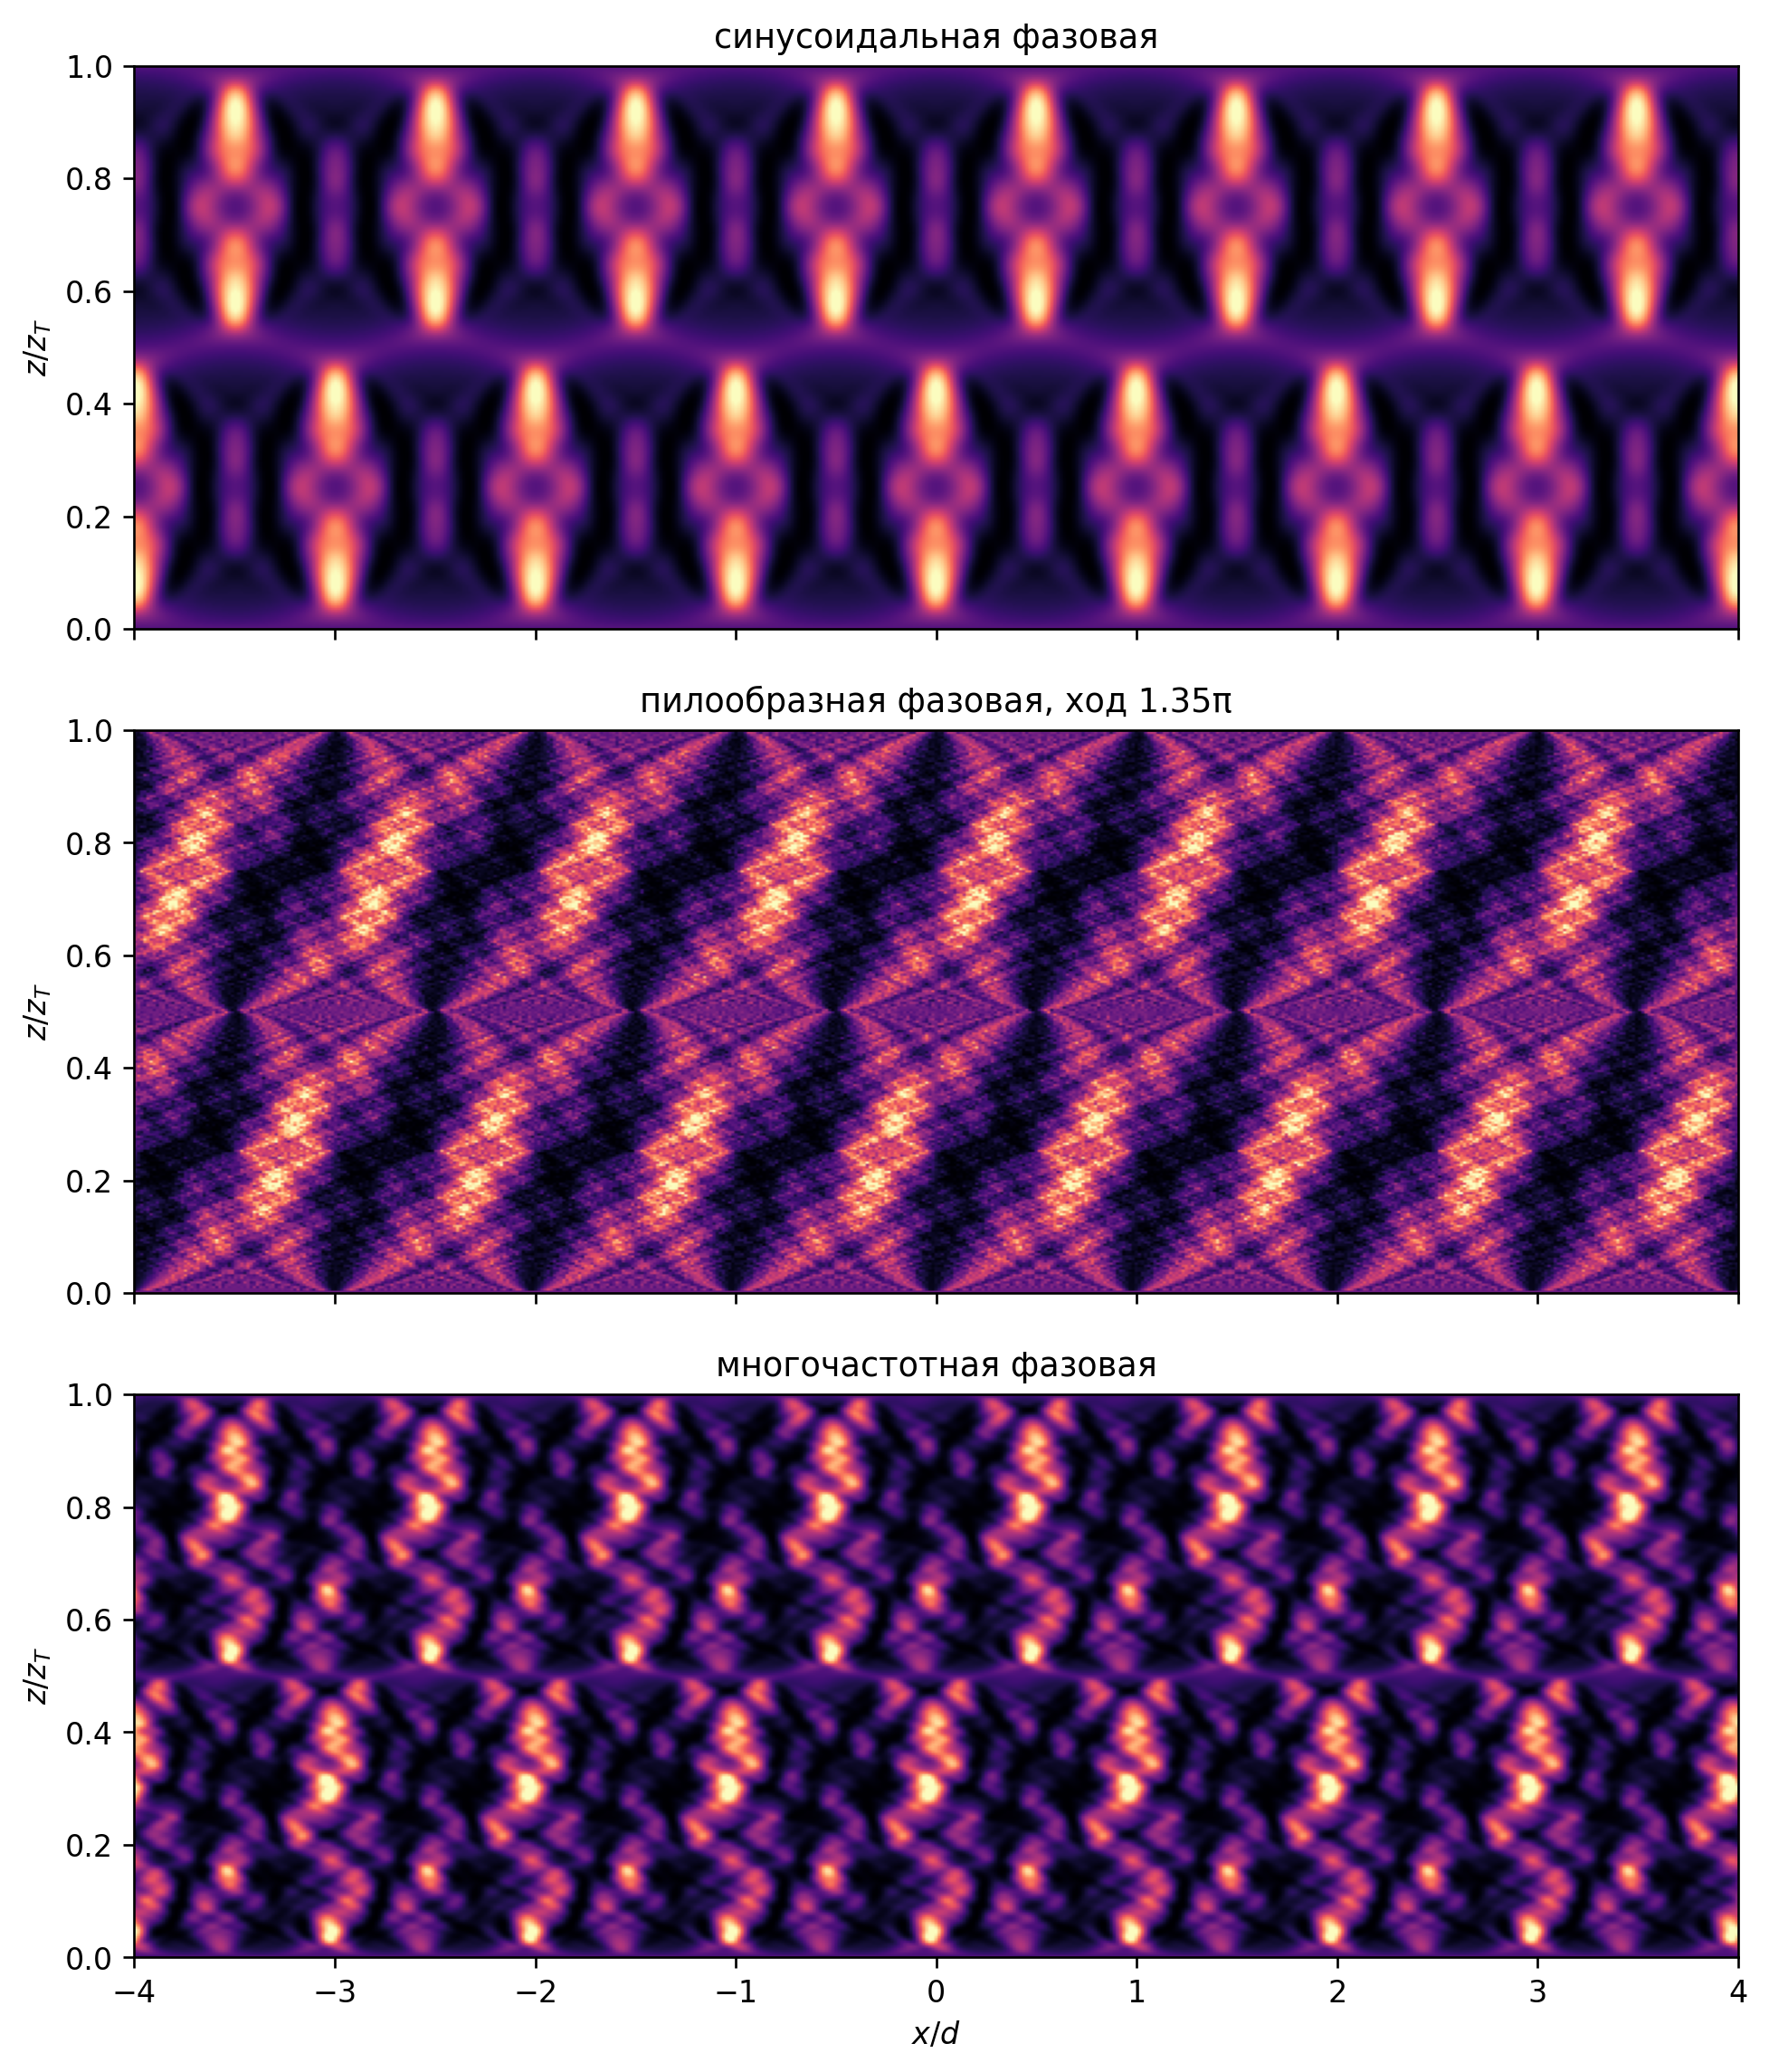
\includegraphics[width=0.98\textwidth]{notebook_phase_gallery.png}
\caption{Сравнение фазовых решеток из ноутбука: синусоидальной, пилообразной и многочастотной. Ровный ход фазы $2\pi$ близок к чистому наклону волнового фронта и может давать почти однородную интенсивность, поэтому для пилообразной решетки выбран неполный ход $1.35\pi$.}
\end{figure}

\subsection{Корреляции, спектры и сравнение моделей}

\begin{figure}[H]
\centering
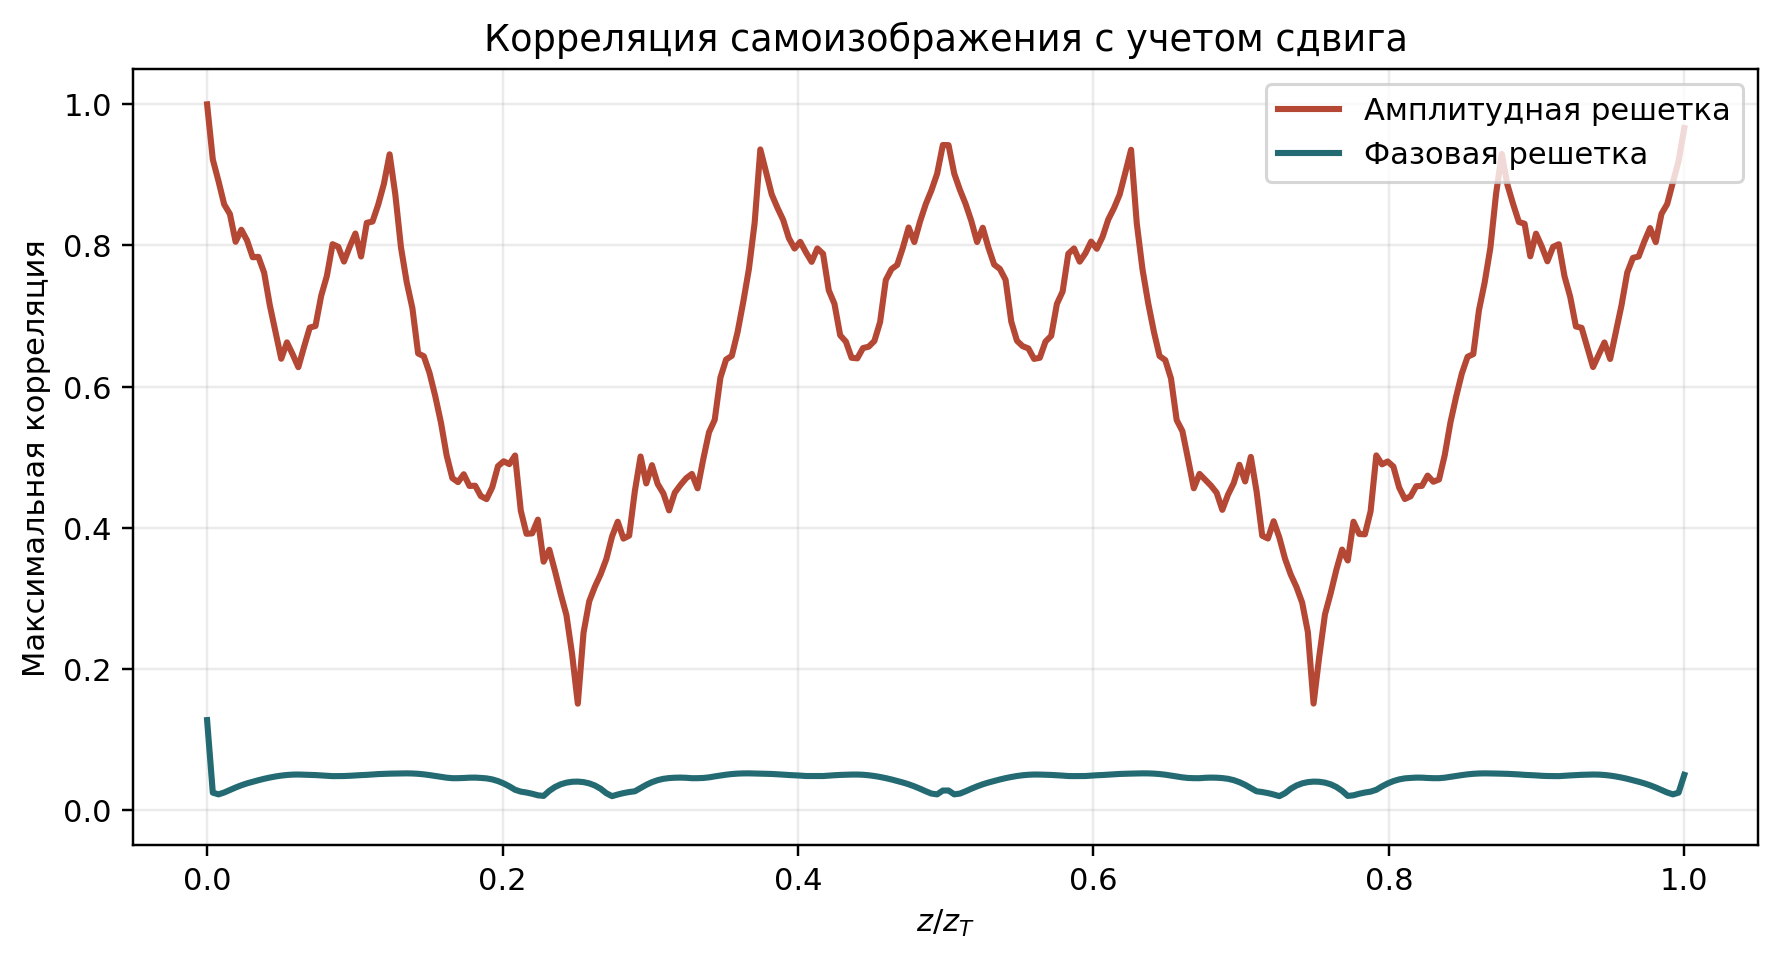
\includegraphics[width=0.82\textwidth]{self_image_correlation.png}
\caption{Корреляция самоизображения как функция $z/z_T$ с учетом оптимального циклического сдвига.}
\end{figure}

\begin{figure}[H]
\centering
\begin{subfigure}{0.44\textwidth}
    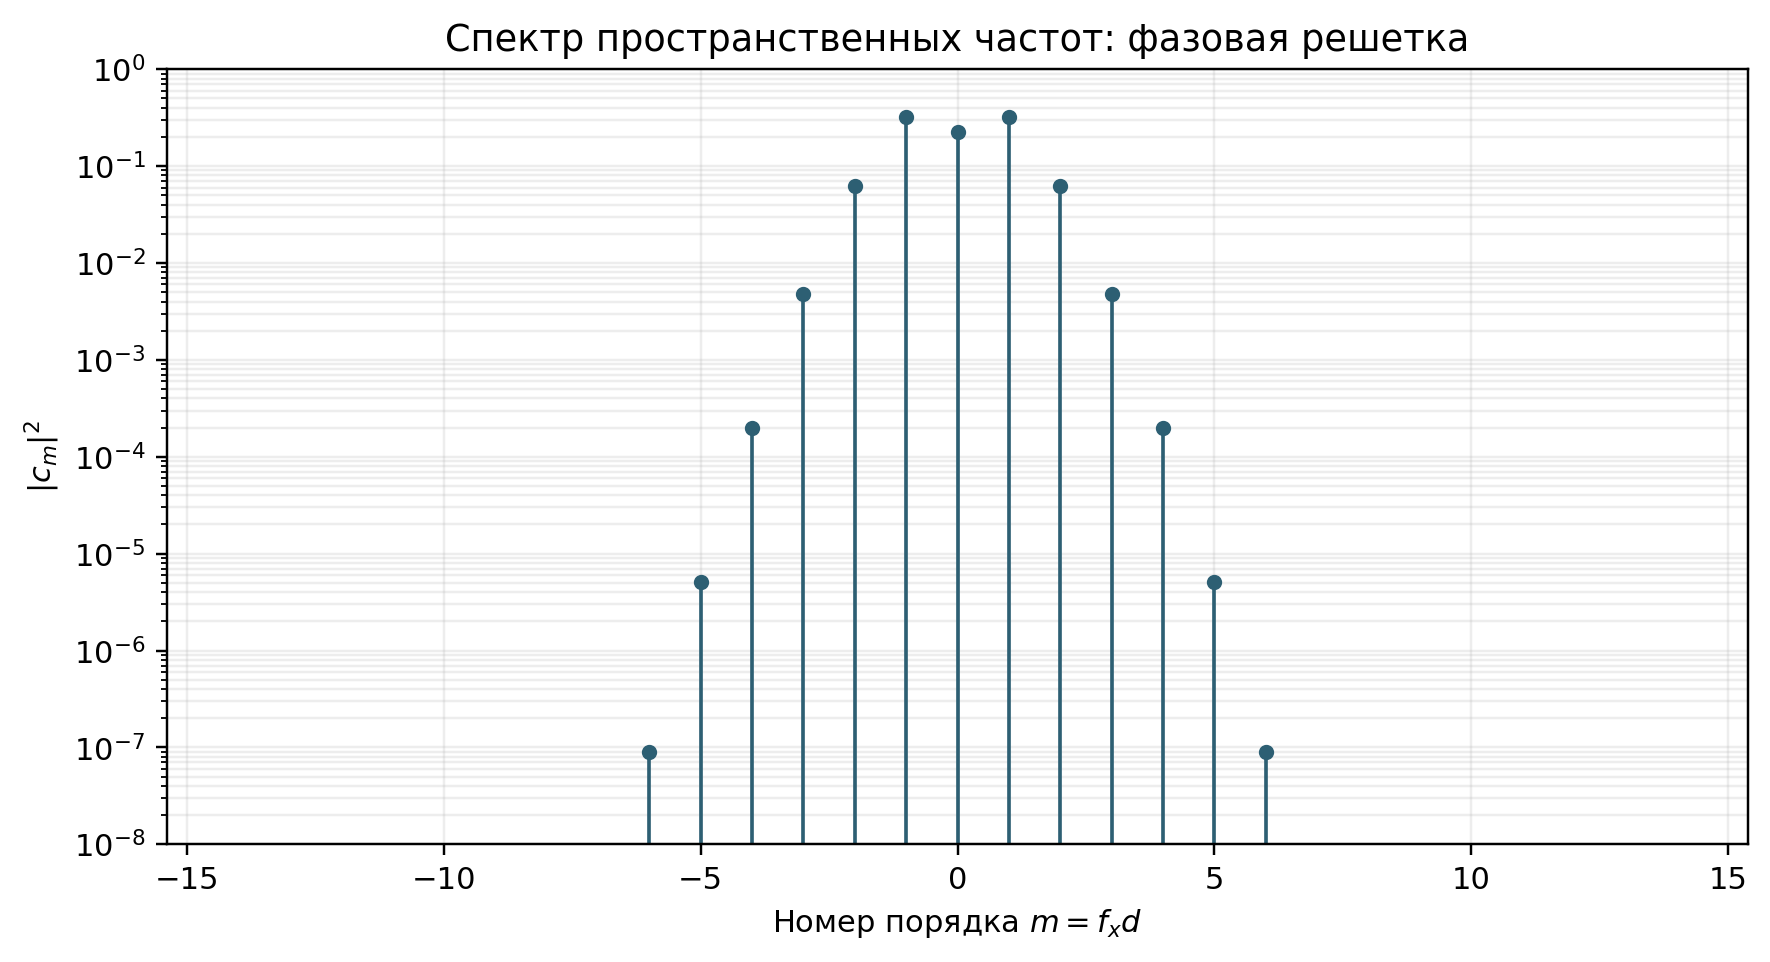
\includegraphics[width=\textwidth]{diffraction_spectrum_phase.png}
    \caption{Фазовая решетка}
\end{subfigure}
\begin{subfigure}{0.44\textwidth}
    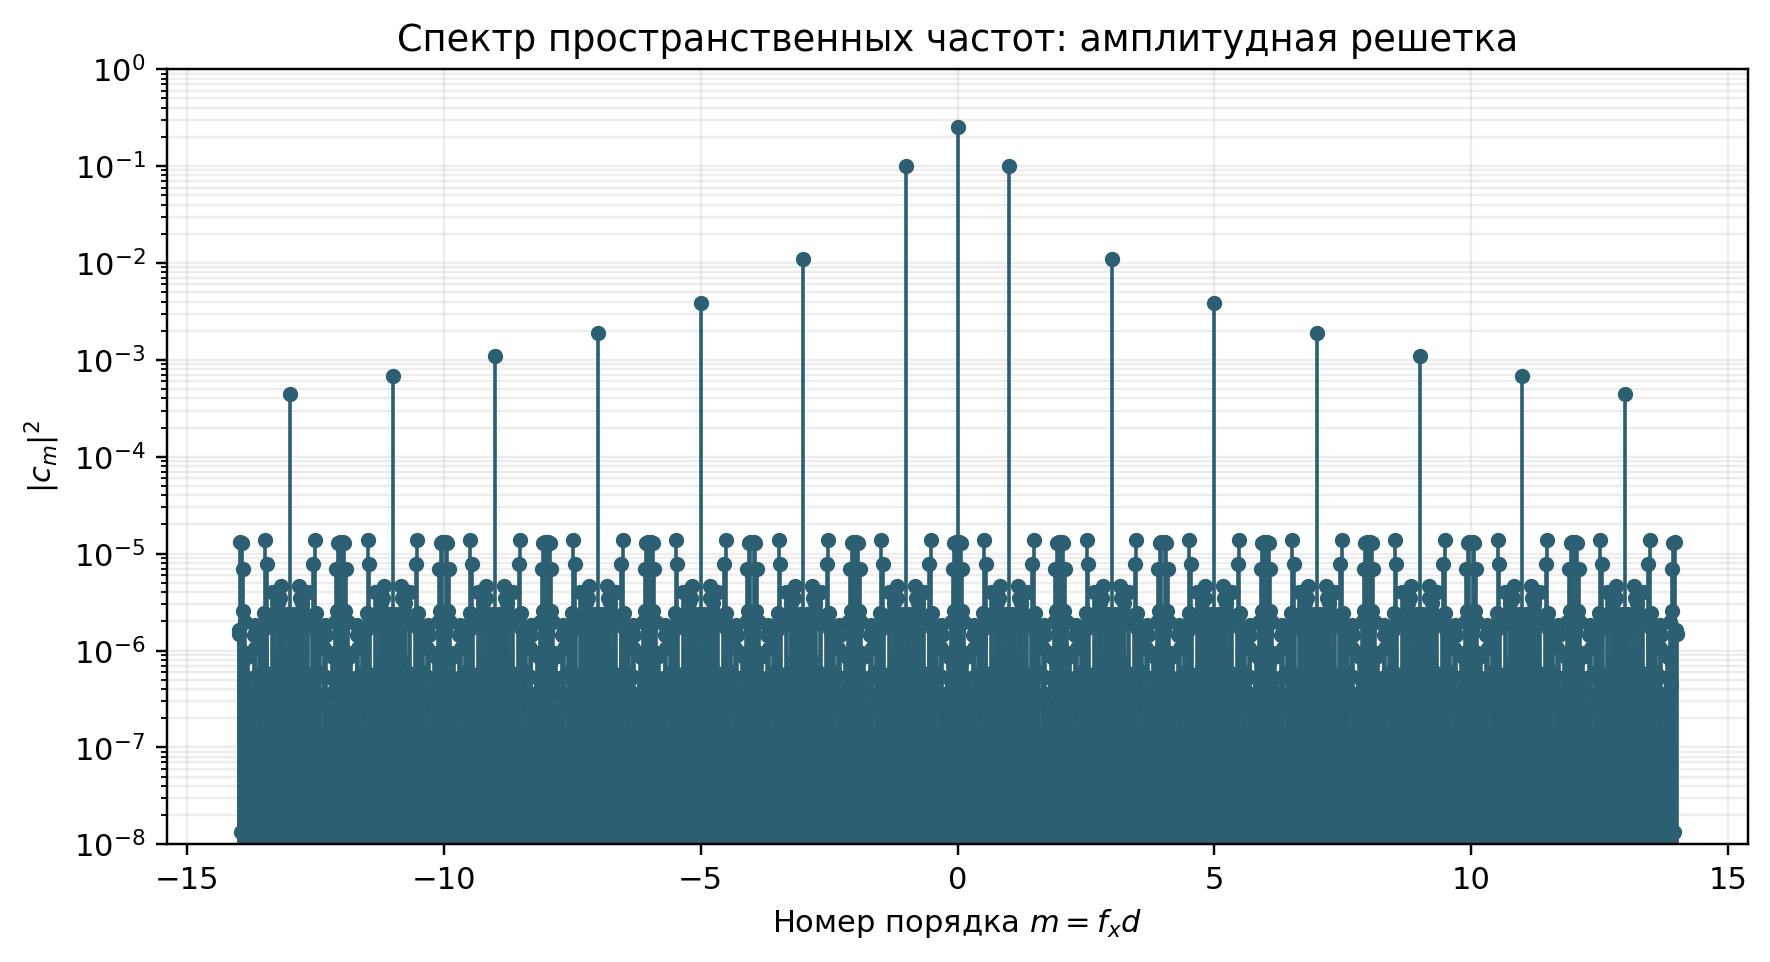
\includegraphics[width=\textwidth]{diffraction_spectrum_amplitude.png}
    \caption{Амплитудная решетка}
\end{subfigure}
\caption{Спектры пространственных частот. Бинарная амплитудная решетка содержит больше высоких гармоник из-за резких краев.}
\end{figure}

\vspace{-2mm}
\begin{center}
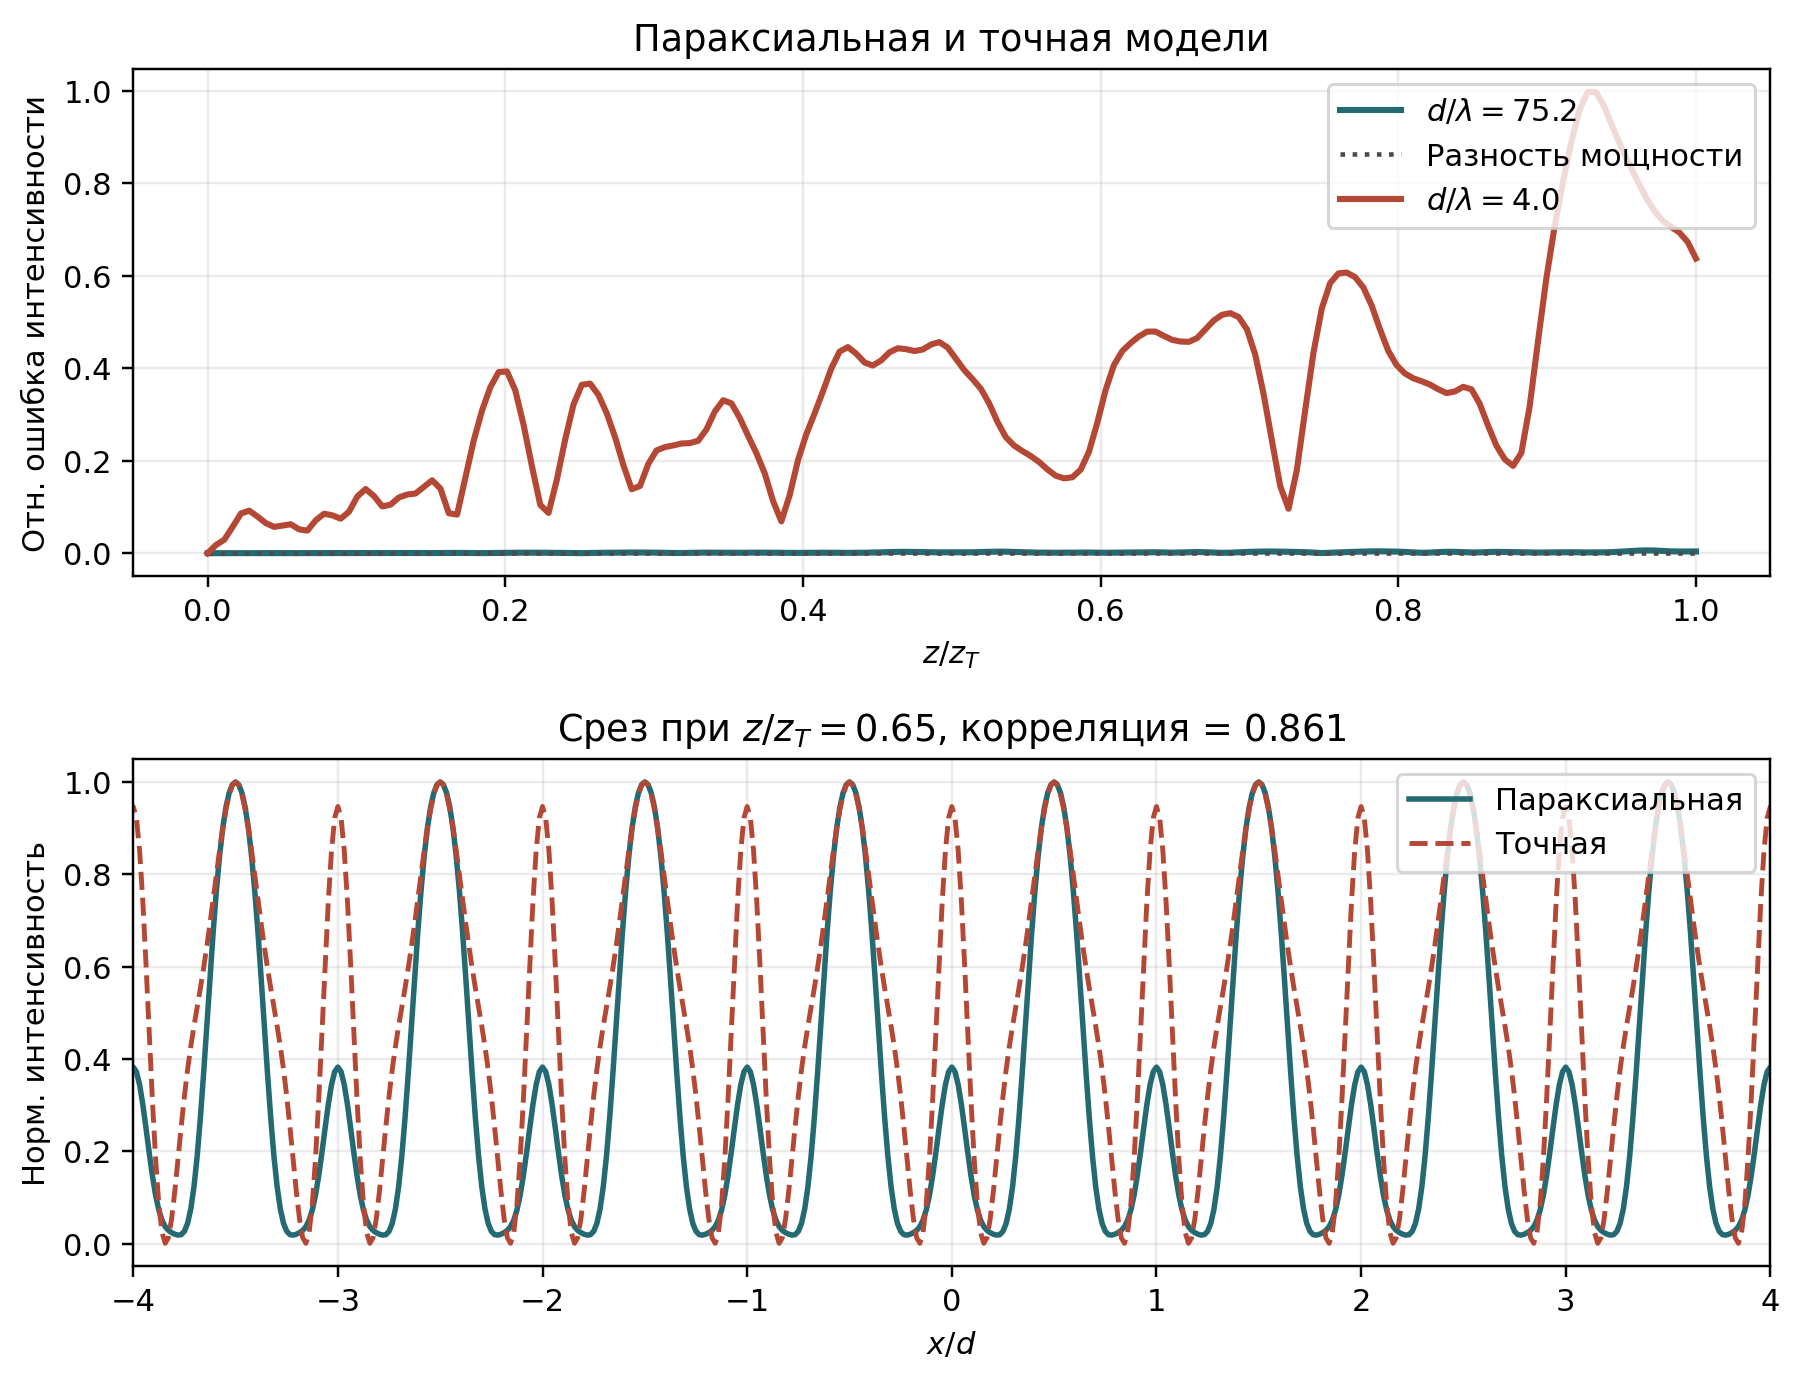
\includegraphics[width=0.55\textwidth]{paraxial_vs_exact.png}
\captionof{figure}{Сравнение параксиальной и точной моделей. При $d/\lambda\gg 1$ отличие мало, при уменьшении периода оно возрастает.}
\end{center}

\begin{figure}[H]
\centering
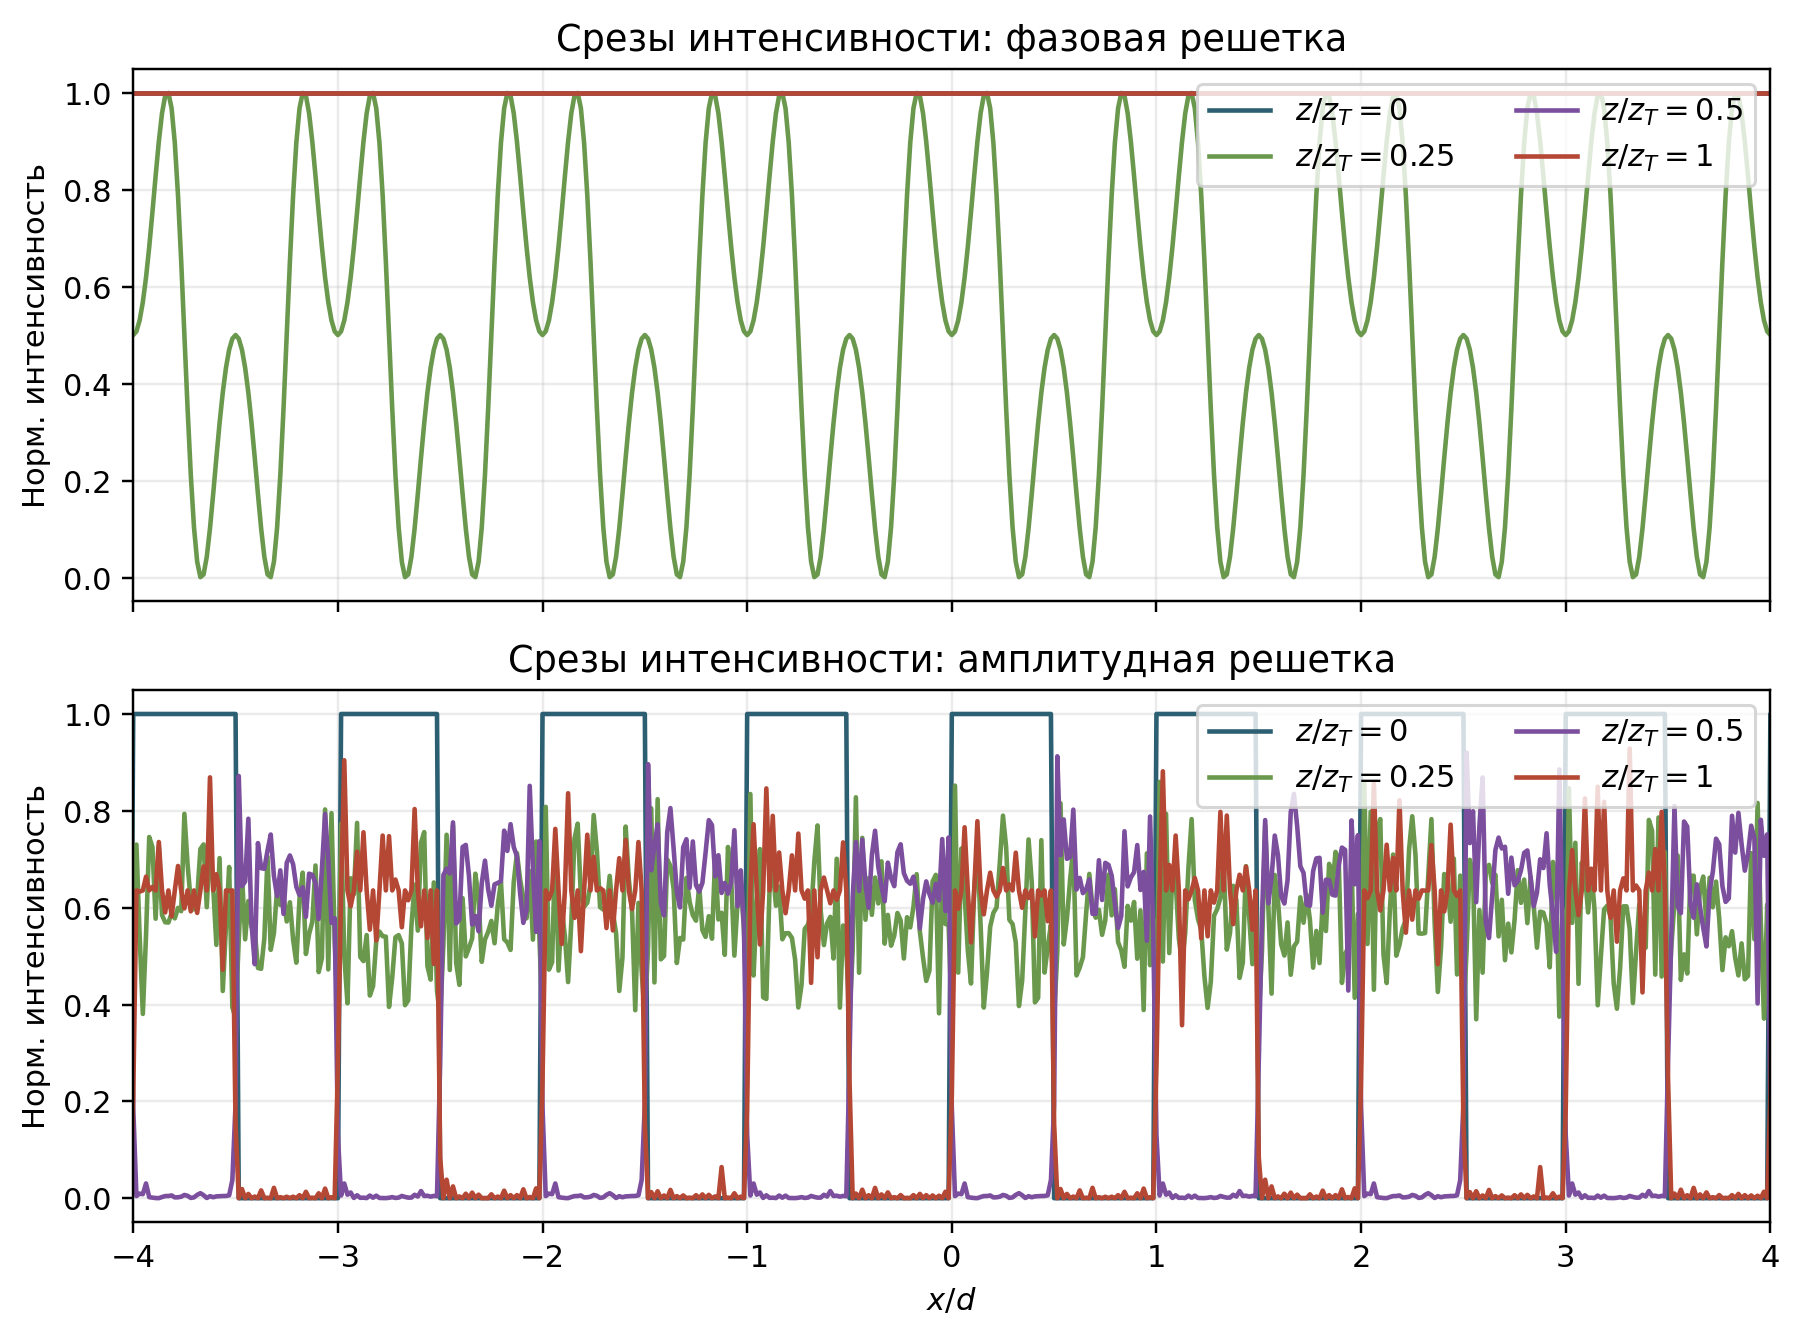
\includegraphics[width=0.9\textwidth]{field_slices.png}
\caption{Срезы интенсивности при $z=0$, $z_T/4$, $z_T/2$ и $z_T$.}
\end{figure}

\section{Проверки корректности}

В проекте реализованы автоматические тесты:
\begin{enumerate}
    \item постоянное поле не должно менять интенсивность при распространении;
    \item полная мощность
    \begin{equation}
        P(z)=\int |U(x,z)|^2\dd x
    \end{equation}
    сохраняется в параксиальной модели;
    \item бинарная амплитудная решетка восстанавливается при $z_T$;
    \item при $z_T/2$ наблюдается высокая корреляция после сдвига на $d/2$;
    \item для решетки
    \begin{equation}
        t(x)=1+m\,\cos\left(\frac{2\pi x}{d}\right)
    \end{equation}
    численное решение сравнивается с аналитическим:
    \begin{equation}
        A(x,z)=
        1+
        m\,\cos\left(\frac{2\pi x}{d}\right)
        \e^{-\ii\pi\lambda z/d^2};
    \end{equation}
    \item результат устойчив к измельчению сетки.
\end{enumerate}

\section{Выводы}

По построенным коврам видно главное свойство эффекта Талбота: периодическая структура не просто размывается после решетки, а периодически собирается снова. Для бинарной амплитудной решетки исходные щели хорошо различимы уже в плоскости решетки; на половине длины Талбота картина появляется со сдвигом на половину периода, а на полной длине Талбота снова совпадает с исходным рисунком.

Фазовая решетка ведет себя иначе: в начальной плоскости интенсивность почти однородна, потому что меняется главным образом фаза. Однако уже при распространении фазовая модуляция превращается в яркие полосы интенсивности. Поэтому фазовые ковры выглядят более насыщенными, особенно для пилообразной, бинарной и многочастотной фазовой ячейки.

Сравнение разных амплитудных ячеек показывает, что форма решетки управляет набором пространственных гармоник. Синусоидальная амплитудная решетка дает более мягкую картину, узкие прямоугольные щели добавляют много высоких порядков и делают дробные изображения резче, широкие щели меняют контраст, а треугольная ячейка сглаживает резкие детали. Многощелевые структуры с двумя, тремя, пятью и семью щелями демонстрируют, что усложнение одного периода не разрушает самовоспроизведение, а добавляет внутренние подструктуры в ковер.

График корреляции подтверждает количественно то, что видно на коврах: вблизи полной длины Талбота возникает сильное самоизображение, а учет циклического сдвига нужен для корректного описания половины длины. Спектры объясняют различия между картинами: чем богаче спектр решетки, тем больше дифракционных порядков участвует в интерференции. Сравнение параксиальной и точной моделей показывает, что при большом периоде относительно длины волны они почти совпадают, а при уменьшении периода различие становится заметным. Поэтому параксиальная модель подходит для обычной геометрии опыта, но точная модель нужна для мелких структур и больших углов дифракции.

\section{Материалы проекта}

Ссылка на репозиторий GitHub:

\vspace{5mm}
\noindent\href{https://github.com/Anana7yk/optics#}{\texttt{github.com/Anana7yk/optics}}
\vspace{4mm}

\noindent\rule{0.92\textwidth}{0.4pt}
\vspace{4mm}

Инструкция по воспроизведению расчетов, запуску тестов, генерации рисунков и открытию Jupyter-ноутбука приведена в файле \texttt{README.md}.

\end{document}
